\documentclass[tikz,border=5mm]{standalone}
\usepackage{tikz}
\usetikzlibrary{calc,patterns}

\begin{document}

% ===== Figure 1: Non-intersecting lattice paths on the cylinder =====
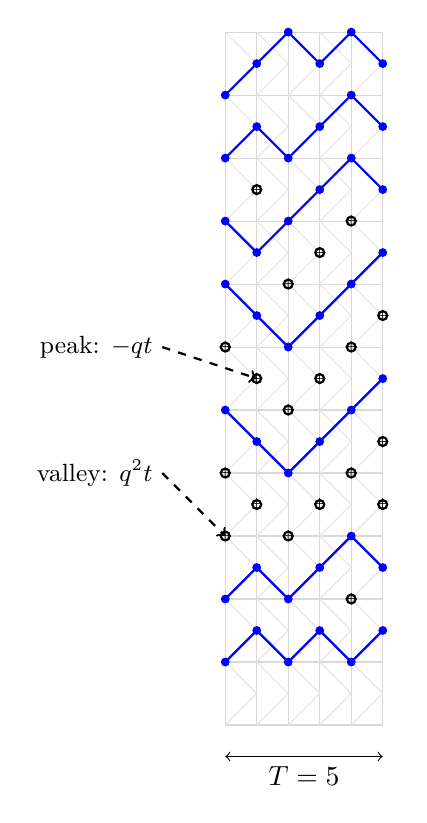
\begin{tikzpicture}[scale=0.4]
  % Draw the lattice grid
  \foreach \x in {0,1,2,3,4,5} {
    \draw[gray!30] (\x,0) -- (\x,22);
  }
  \foreach \y in {0,2,4,6,8,10,12,14,16,18,20,22} {
    \draw[gray!30] (0,\y) -- (5,\y);
  }

  % Draw diagonal grid lines (triangular lattice)
  \foreach \y in {1,3,5,7,9,11,13,15,17,19,21} {
    \foreach \x in {0,1,2,3,4} {
      \draw[gray!20] (\x,\y-1) -- (\x+1,\y);
      \draw[gray!20] (\x,\y+1) -- (\x+1,\y);
    }
  }

  % Path 1: (1,0,1,0,1), y_0 = 2
  \draw[thick,blue] (0,2) -- (1,3) -- (2,2) -- (3,3) -- (4,2) -- (5,3);
  \foreach \x/\y in {0/2,1/3,2/2,3/3,4/2,5/3} {
    \fill[blue] (\x,\y) circle (4pt);
  }

  % Path 2: (1,0,1,1,0), y_0 = 4
  \draw[thick,blue] (0,4) -- (1,5) -- (2,4) -- (3,5) -- (4,6) -- (5,5);
  \foreach \x/\y in {0/4,1/5,2/4,3/5,4/6,5/5} {
    \fill[blue] (\x,\y) circle (4pt);
  }

  % Path 3: (0,0,1,1,1), y_0 = 10
  \draw[thick,blue] (0,10) -- (1,9) -- (2,8) -- (3,9) -- (4,10) -- (5,11);
  \foreach \x/\y in {0/10,1/9,2/8,3/9,4/10,5/11} {
    \fill[blue] (\x,\y) circle (4pt);
  }

  % Path 4: (0,0,1,1,1), y_0 = 14
  \draw[thick,blue] (0,14) -- (1,13) -- (2,12) -- (3,13) -- (4,14) -- (5,15);
  \foreach \x/\y in {0/14,1/13,2/12,3/13,4/14,5/15} {
    \fill[blue] (\x,\y) circle (4pt);
  }

  % Path 5: (0,1,1,1,0), y_0 = 16
  \draw[thick,blue] (0,16) -- (1,15) -- (2,16) -- (3,17) -- (4,18) -- (5,17);
  \foreach \x/\y in {0/16,1/15,2/16,3/17,4/18,5/17} {
    \fill[blue] (\x,\y) circle (4pt);
  }

  % Path 6: (1,0,1,1,0), y_0 = 18
  \draw[thick,blue] (0,18) -- (1,19) -- (2,18) -- (3,19) -- (4,20) -- (5,19);
  \foreach \x/\y in {0/18,1/19,2/18,3/19,4/20,5/19} {
    \fill[blue] (\x,\y) circle (4pt);
  }

  % Path 7: (1,1,0,1,0), y_0 = 20
  \draw[thick,blue] (0,20) -- (1,21) -- (2,22) -- (3,21) -- (4,22) -- (5,21);
  \foreach \x/\y in {0/20,1/21,2/22,3/21,4/22,5/21} {
    \fill[blue] (\x,\y) circle (4pt);
  }

  % White (unoccupied) vertices - surface cubes
  \foreach \x/\y in {0/6,0/8,0/12,1/7,1/11,1/17,2/6,2/10,2/14,3/7,3/11,3/15,4/4,4/8,4/12,4/16,5/7,5/9,5/13} {
    \draw[thick] (\x,\y) circle (4pt);
    \node at (\x,\y) {\tiny +};
  }

  % Label valley and peak cubes
  \draw[->,thick,dashed] (-2,8) -- (0,6);
  \node[left] at (-2,8) {\small valley: $q^2t$};

  \draw[->,thick,dashed] (-2,12) -- (1,11);
  \node[left] at (-2,12) {\small peak: $-qt$};

  % Period indicator
  \draw[<->] (0,-1) -- (5,-1);
  \node[below] at (2.5,-1) {$T=5$};

\end{tikzpicture}

\vspace{1cm}

% ===== Figure 2: Rhombus tiling on the cylinder =====
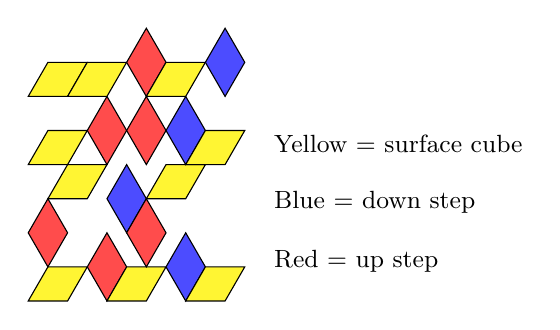
\begin{tikzpicture}[scale=0.5]
  % Define rhombus shapes
  \newcommand{\redup}[2]{% red tile (up step)
    \fill[red!70] (#1,#2) -- (#1+0.5,#2+0.866) -- (#1+1,#2) -- (#1+0.5,#2-0.866) -- cycle;
    \draw[black] (#1,#2) -- (#1+0.5,#2+0.866) -- (#1+1,#2) -- (#1+0.5,#2-0.866) -- cycle;
  }
  \newcommand{\bluedown}[2]{% blue tile (down step)
    \fill[blue!70] (#1,#2) -- (#1+0.5,#2+0.866) -- (#1+1,#2) -- (#1+0.5,#2-0.866) -- cycle;
    \draw[black] (#1,#2) -- (#1+0.5,#2+0.866) -- (#1+1,#2) -- (#1+0.5,#2-0.866) -- cycle;
  }
  \newcommand{\yellowflat}[2]{% yellow tile (white vertex / surface cube)
    \fill[yellow!80] (#1,#2) -- (#1+1,#2) -- (#1+1.5,#2+0.866) -- (#1+0.5,#2+0.866) -- cycle;
    \draw[black] (#1,#2) -- (#1+1,#2) -- (#1+1.5,#2+0.866) -- (#1+0.5,#2+0.866) -- cycle;
  }

  % Build a sample tiling (simplified version showing the structure)
  % Row 0-1
  \yellowflat{0}{0}
  \redup{1.5}{0.866}
  \yellowflat{2}{0}
  \bluedown{3.5}{0.866}
  \yellowflat{4}{0}

  % Row 1-2
  \redup{0}{1.732}
  \yellowflat{0.5}{2.598}
  \bluedown{2}{2.598}
  \redup{2.5}{1.732}
  \yellowflat{3}{2.598}

  % Row 2-3
  \yellowflat{0}{3.464}
  \redup{1.5}{4.33}
  \redup{2.5}{4.33}
  \bluedown{3.5}{4.33}
  \yellowflat{4}{3.464}

  % More rows to show periodic structure
  \yellowflat{0}{5.196}
  \yellowflat{1}{5.196}
  \redup{2.5}{6.062}
  \yellowflat{3}{5.196}
  \bluedown{4.5}{6.062}

  % Legend
  \node[right] at (6,1) {\small Red = up step};
  \node[right] at (6,2.5) {\small Blue = down step};
  \node[right] at (6,4) {\small Yellow = surface cube};

\end{tikzpicture}

\vspace{1cm}

% ===== Figure 3: Growth diagram for cylindric partition =====
% Shows the sequence of partitions as Young diagrams
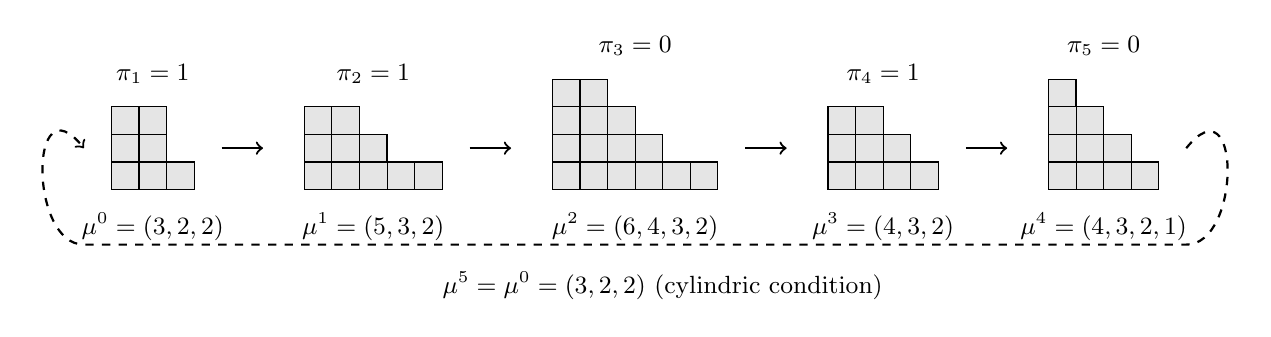
\begin{tikzpicture}[scale=0.35]

  % mu^0 = (3,2,2)
  \begin{scope}[shift={(0,0)}]
    \draw[fill=gray!20] (0,0) rectangle (3,1);
    \draw[fill=gray!20] (0,1) rectangle (2,2);
    \draw[fill=gray!20] (0,2) rectangle (2,3);
    \draw (0,0) grid (3,1);
    \draw (0,1) grid (2,3);
    \node[below] at (1.5,-0.5) {\small $\mu^0=(3,2,2)$};
    \node[above] at (1.5,3.5) {\small $\pi_1=1$};
  \end{scope}

  % Arrow
  \draw[->,thick] (4,1.5) -- (5.5,1.5);

  % mu^1 = (5,3,2)
  \begin{scope}[shift={(7,0)}]
    \draw[fill=gray!20] (0,0) rectangle (5,1);
    \draw[fill=gray!20] (0,1) rectangle (3,2);
    \draw[fill=gray!20] (0,2) rectangle (2,3);
    \draw (0,0) grid (5,1);
    \draw (0,1) grid (3,2);
    \draw (0,2) grid (2,3);
    \node[below] at (2.5,-0.5) {\small $\mu^1=(5,3,2)$};
    \node[above] at (2.5,3.5) {\small $\pi_2=1$};
  \end{scope}

  % Arrow
  \draw[->,thick] (13,1.5) -- (14.5,1.5);

  % mu^2 = (6,4,3,2)
  \begin{scope}[shift={(16,0)}]
    \draw[fill=gray!20] (0,0) rectangle (6,1);
    \draw[fill=gray!20] (0,1) rectangle (4,2);
    \draw[fill=gray!20] (0,2) rectangle (3,3);
    \draw[fill=gray!20] (0,3) rectangle (2,4);
    \draw (0,0) grid (6,1);
    \draw (0,1) grid (4,2);
    \draw (0,2) grid (3,3);
    \draw (0,3) grid (2,4);
    \node[below] at (3,-0.5) {\small $\mu^2=(6,4,3,2)$};
    \node[above] at (3,4.5) {\small $\pi_3=0$};
  \end{scope}

  % Arrow
  \draw[->,thick] (23,1.5) -- (24.5,1.5);

  % mu^3 = (4,3,2)
  \begin{scope}[shift={(26,0)}]
    \draw[fill=gray!20] (0,0) rectangle (4,1);
    \draw[fill=gray!20] (0,1) rectangle (3,2);
    \draw[fill=gray!20] (0,2) rectangle (2,3);
    \draw (0,0) grid (4,1);
    \draw (0,1) grid (3,2);
    \draw (0,2) grid (2,3);
    \node[below] at (2,-0.5) {\small $\mu^3=(4,3,2)$};
    \node[above] at (2,3.5) {\small $\pi_4=1$};
  \end{scope}

  % Arrow
  \draw[->,thick] (31,1.5) -- (32.5,1.5);

  % mu^4 = (4,3,2,1)
  \begin{scope}[shift={(34,0)}]
    \draw[fill=gray!20] (0,0) rectangle (4,1);
    \draw[fill=gray!20] (0,1) rectangle (3,2);
    \draw[fill=gray!20] (0,2) rectangle (2,3);
    \draw[fill=gray!20] (0,3) rectangle (1,4);
    \draw (0,0) grid (4,1);
    \draw (0,1) grid (3,2);
    \draw (0,2) grid (2,3);
    \draw (0,3) grid (1,4);
    \node[below] at (2,-0.5) {\small $\mu^4=(4,3,2,1)$};
    \node[above] at (2,4.5) {\small $\pi_5=0$};
  \end{scope}

  % Arrow (wrapping back)
  \draw[->,thick,dashed] (39,1.5) .. controls (41,4) and (41,-2) .. (39,-2) -- (-1,-2) .. controls (-3,-2) and (-3,4) .. (-1,1.5);
  \node at (20,-3.5) {\small $\mu^5 = \mu^0 = (3,2,2)$ (cylindric condition)};

\end{tikzpicture}

\vspace{1cm}

% ===== Figure 4: Profile and inversions for Conjecture 2.7 context =====
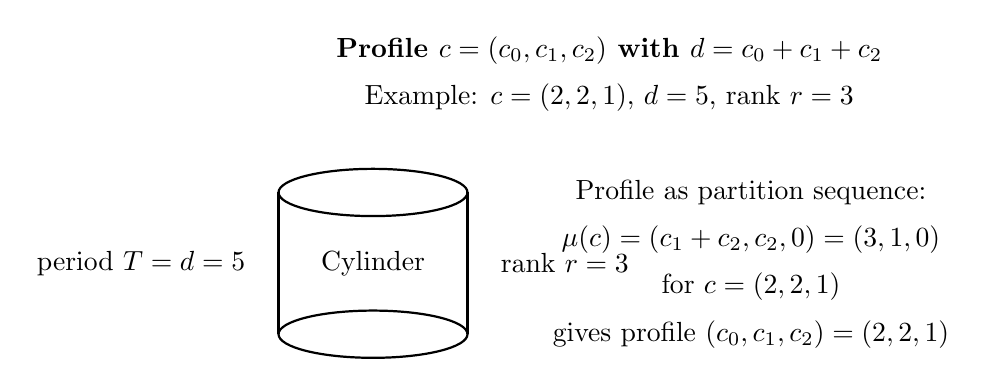
\begin{tikzpicture}[scale=0.6]
  % Title
  \node at (5,6) {\textbf{Profile $c = (c_0, c_1, c_2)$ with $d = c_0 + c_1 + c_2$}};

  % Example: c = (2,2,1), d = 5, rank r = 3
  \node at (5,5) {Example: $c = (2,2,1)$, $d = 5$, rank $r = 3$};

  % Draw the cylindric structure schematically
  \draw[thick] (0,0) ellipse (2 and 0.5);
  \draw[thick] (0,3) ellipse (2 and 0.5);
  \draw[thick] (-2,0) -- (-2,3);
  \draw[thick] (2,0) -- (2,3);

  % Label
  \node at (0,1.5) {Cylinder};
  \node[left] at (-2.5,1.5) {period $T=d=5$};
  \node[right] at (2.5,1.5) {rank $r=3$};

  % The profile sequence
  \begin{scope}[shift={(6,0)}]
    \node at (2,3) {Profile as partition sequence:};
    \node at (2,2) {$\mu(c) = (c_1+c_2, c_2, 0) = (3,1,0)$};
    \node at (2,1) {for $c = (2,2,1)$};
    \node at (2,0) {gives profile $(c_0, c_1, c_2) = (2,2,1)$};
  \end{scope}

\end{tikzpicture}

\end{document}
